\subsection{Turning wind}
%

% - Purpose & Problem description:
%     These first two parts give reader short details about the test case,
%     the physical phenomena involved and specify how the numerical solution will be validated
%
\subsubsection{Purpose}
%
This test case shows how Tomawac calculate the spectrum when there is a wind that is turning. It illustrates the phenomena of white capping and quadruplet interactions.  This document is a short translation of the french 'doc' version. One can find more details in {\it turning\_wind/doc/turningwind.doc}

%
\subsubsection{Description of the problem}
%
The domain is homogeneous, The depth is infinite, the wind given at 10m is homogeneous  propagation step is inhibited and no boundary condition are given.
So the domain of computation can be reduced to a few points as the solution is homogeneous and finally we focus on only one of them. The domain is finally very simple (see Figure \ref{mailTW})
% - Reference:
%     This part gives the reference solution we are comparing to and
%     explicits the analytical solution when available;


% - Physical parameters:
%     This part specifies the geometry, details all the physical parameters
%     used to describe both porous media (soil model in particularly) and
%     solute characteristics (dispersion/diffusion coefficients, soil <=> pollutant interactions...)
%
%
\subsubsection{Physical parameters}
%
The modulus of the wind is constant equalled to 20 m/s. Initially the direction is set to 90 degree, (which mean that $U_Y$ is null). This is maintained till the peak frequency reach the double of its equilibrium value (peak frequency of Pierson-Moskowitz). This occurs after 28800s (8h), at this time we change the direction of wind for 30 degrees (a rotation of 60 degrees). All the value of the wind are read in a file called {\it wind.slf   }.
% - Geometry and Mesh:
%     This part describes the mesh used in the computation
%
%
\subsubsection{Geometry and Mesh}
%
The domain is a square of 2km
The mesh is very simple as there are 5 nodes and 4 triangles
\begin{figure} [!h]
\centering
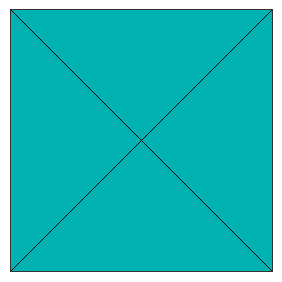
\includegraphics[scale = 0.65]{maillage.png}
 \caption{Mesh of the domain}
\label{mailTW}
\end{figure}
% - Initial and boundary conditions:
%     This part details both initial and boundary conditions used to simulate the case
%
%
\subsubsection{Initial and Boundary Conditions}
%
Initial conditions are imposed homogeneous on the domain with the option 4, with a phillips constant of 0.024 an initial peak frequency of 0.3  and an initial peak factor of 1.  The initial directionnal spread is set to one and the initial main direction to 90 degree (like the wind).
Those value has been set to be identical to the Vledder study \cite{vledder}

Nothing is imposed at the boundaries.
% - Numerical parameters:
%     This part is used to specify the numerical parameters used
%     (adaptive time step, mass-lumping when necessary...)
%
%
\subsubsection{Numerical parameters}
Time duration is set to 115200s (32h), time step is equal to 900s, the spectro-angular mesh has 12 angles and 26 frequences spread on a geometric progression common ratio 1.1 with a minimum of 0.04177248.

% - Results:
%     We comment in this part the numerical results against the reference ones,
%     giving understanding keys and making assumptions when necessary.
%
%
\subsubsection{Results}
%
We present here the results only for the rotation of 60 degrees as it is the effective rotation that is done in the case. Initially there were 3 rotations one of 90 and one of 30. The results for those rotations are described in \cite{valid10TW}.

At the moment when the direction change the established swell is going to interact with the wave induced by the new direction of wind. Three phenomenas occur in that process.
\begin {itemize}
\item Wind contribution to the energy that will raise the new wave.
\item Attenuation of the swell part of the spectrum
\item Non linear interactions between swell and wind's sea.
\end{itemize}

The results of Tomawac are compared to simulations made by two differents code. EXACT-NL and WAM-cycle 3 (voir \cite{vledder}). The figure  \ref{resturnwind} shows that there are good agreements of Tomawac results compared to other simulations. One can denote that spectrum tail factor can be sensitive. During the first 4 hours a factor of 4 is better but after that time a factor of 5 is better.

Let us remark that those are old results and a new simulation with new linear terms might give better results.

\begin{figure} [!h]
\centering
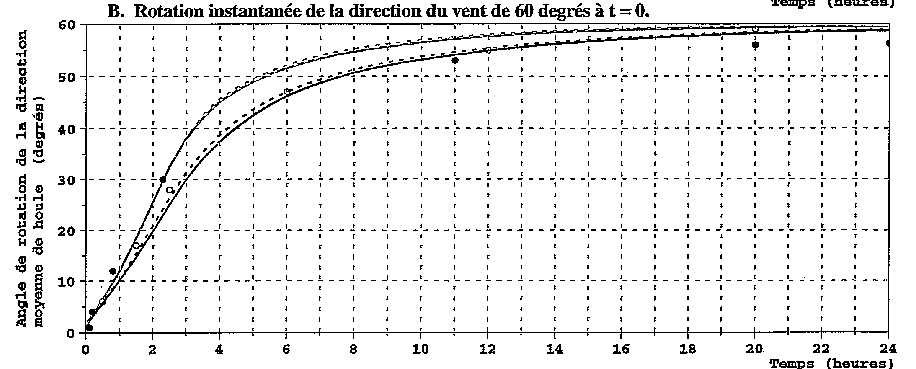
\includegraphics[scale = 0.45]{resuTW60.png}
 \caption{Comparison of direction of wave with time after a direction change of 60 degree at t=0. Simulations are made for differents spectrum tail factor and different initial spectrum}
\label{resturnwind}
\end{figure}

% Here is an example of how to include the graph generated by validateTELEMAC.py
% They should be in test_case/img
%\begin{figure} [!h]
%\centering
%\includegraphics[scale=0.3]{mygraph.png}
% \caption{mycaption}\label{mylabel}
%\end{figure}

